% a sample file for Journal of Quantum Information and Computation (QIC) in 
% LaTex2e by inputing macro file "qic.sty" with command \usepackage{qic}, 
% all the macros have been defined in the style file, so it is no need to 
% put many macros at the beginning of the text file  

\documentclass[twoside]{article}
\usepackage{qic,epsfig}
\usepackage{braket}
\usepackage{bm}
\usepackage{amssymb}
\usepackage{amsmath}
\usepackage{qcircuit}
\usepackage{mathtools}
\usepackage{verbatim}
\usepackage{breqn}
\usepackage{tikz}
\usetikzlibrary{arrows.meta}

\textwidth=5.6truein
\textheight=8.0truein

\renewcommand{\thefootnote}{\fnsymbol{footnote}}  %use symbolic footnote

%%%%%%% starting the text file 

\begin{document}
\setlength{\textheight}{8.0truein}    %FOR 2ND PAGE ONWARDS

\runninghead{Mapping Fermions to Qubits  $\ldots$}
            {Oliver O'Brien $\ldots$}

\normalsize\textlineskip
\thispagestyle{empty}
\setcounter{page}{1}

%\copyrightheading{Vol.}{No.}{Year}{Page Nos.}
\copyrightheading{0}{0}{2003}{000--000}

\vspace*{0.88truein}

\alphfootnote

\fpage{1}

\centerline{\bf
%%%%%%%%%%%%%%%%%%%%%
%Put in titiles here
%%%%%%%%%%%%%%%%%%%%%
MAPPING FERMIONS TO QUBITS}
\vspace*{0.37truein}
\centerline{\footnotesize
%%%%%%%%%%%%%%%%%%%%%%%%%%%%%%%%%%%%
%put authors' name and address here
%%%%%%%%%%%%%%%%%%%%%%%%%%%%%%%%%%%%
OLIVER O'BRIEN}
\vspace*{0.015truein}
\centerline{\footnotesize\it DAMTP, Centre for Mathematical Sciences, University of Cambridge, Cambridge CB30WA, UK}
\baselineskip=10pt
\centerline{\footnotesize\it Christ's College, Cambridge, UK}
\vspace*{0.225truein}
\publisher{(received date)}{(revised date)}

\vspace*{0.21truein}

%% \abstracts{first paragraph}{second paragraph}{third paragraph}
%% If there is only one paragraph, just keep the second and third empty 
%% like the following one 
\abstracts{
%%%%%%%%%%%%%%%%%%%%
% put abstract here
%%%%%%%%%%%%%%%%%%%%
Your abstract goes here. 
}{}{}

\vspace*{10pt}

\keywords{The contents of the keywords}
\vspace*{3pt}
\communicate{to be filled by the Editorial}

\vspace*{1pt}\textlineskip    %) USE THIS MEASUREMENT WHEN THERE IS
   %) A SECTION HEADING
%\vspace*{-0.5pt}
%\noindent
%%%%%%%%%%%%%%%%%%%%%%%%%%%%%%%%
%put the text of the paper here
%%%%%%%%%%%%%%%%%%%%%%%%%%%%%%%%
\section{Introduction}
"Nature isn't classical, dammit, and if you want to make a simulation of nature, you'd better make it quantum mechanical, and by golly it's a wonderful problem, because it doesn't look so easy." - \textsl{Dr Richard Feynman} \cite{feynmann} \\\\
Ever since Dr Richard Feynman said these famous words at the end of his keynote speech in 1982, one of the main tasks facing quantum computers has been simulating quantum systems. Intuitively a quantum computer should be able to handle this problem better than a classic computer as they operate within the same bizarre world of entanglement and superposition. However, there are many challenges to overcome before quantum advantage can be achieved in this field. We will consider one such challenge in this essay: the optimum mapping scheme from fermions to qubits.\\\\
One of the most common classes of quantum systems we wish to simulate are those composed of fermions. In order to simulate these particles we must find a representation for them in terms a quantum computer can process, that is qubits and qubit operators. This poses a fundamental issue as fermions exhibit the non-local property of anti-commutation (\textbf{need to explain why it is non-local}), whereas qubits are independent local units. Therefore a non-trival mapping scheme which introduces this non-local behaviour is necessary.\\\\
The first such mapping, the \textbf{Jordan-Wigner Transformation}, was invented nearly a century ago \cite{originalJordanWigner}, and we will introduce it in Section~\ref{jordan-wigner_section}. More recently, a number of new mappings have been developed including the \textbf{Bravyi-Kitaev map} and the \textbf{Derby-Klassen map}, which will be discussed in Section~\ref{bravyi-kitaev_section} and Section~\ref{derby-klassen_section} respectively. Furthermore, recent research \cite{fermionicEncoding} has shown that the \textbf{fermionic enumeration} scheme used in a given mapping (we consider solely the Jordan-Wigner case) offers potential for increased locality with no additional resources. This is elaborated on in Section~\ref{fermionic-enumeration_section}.\\\\
It is important to consider how these mappings impact upon the fermionic simulation techniques used. Therefore, in Section~\ref{applications_section} we will discuss how VQE and phase estimation can both be used to estimate the ground state energy of a system . Finally,  in Section~\ref{comparision_section} we will compare the relative performance of these mappings in real-world applications (using simulated quantum computers).

\section{Applications to fermionic systems}\label{applications_section}
\subsection{Estimating ground state energies}\label{vqe_section}
Computing the ground state energy of a Hamiltonian is generally the first step in computing the energetic properties of molecules and materials \cite{vqe}. Chemists have developed classical computational models for estimating the ground state, however, they all rely on approximations. Quantum computing opens up the potential for an exact (\textit{full configuration interaction}) approach, which is unfeasible on a classical computer where it scales exponentially (\textbf{verify this is true}) in the number of fermionic modes.
\subsubsection{Variational Quantum Eigensolver}
A VQE provides an upper bound on the ground state energy of a Hamiltonian by utilising the variational principle:
\begin{equation}
        \frac{\bra{\psi} \hat H \ket{\psi}}{\braket{\psi | \psi}} \geq E_0 \>\>\>\> \forall \> \ket{\psi}\in \mathcal{H}
\end{equation}
The algorithm consists of two stages. First a variational ansatz is initialised based on a set of parameters $\bm \theta$. Then, the Hamiltonian is measured a number of times, and the parameters of the ansatz are varied until a minimum is found. This is an example of a variational quantum algorithm, which performs a classical optimisation over a quantum oracle (\textbf{is this a correct description}). By exporting lots of the work to a classical computer, VQEs are one of the quantum algorithms that are achievable in the NISQ (Noisy Intermediate-scale Quantum) era.\\\\ 
The preparation of ansatz can be done without any regard for fermions or what underlying wavefunction it represents. Generally a given circuit structure is picked with some of the gates depending upon the parameters (i.e. an $R_z(\theta)$ gate). However, there are some schemes for preparing ansatz that correlate to known wavefunctions, so the wavefunction corresponding to the minimum energy estimate can be found (\textbf{check this is true, find example and see if mapping is important} - Unitary Coupled Cluser - gaussian).\\\\
It is in the measurement of the Hamiltonian that the mapping becomes important. The Hamiltonian in question will be a combination of fermionic raising and lowering operators, so needs to be mapped to a combination of Pauli operators that can be measured on a quantum computer. \textbf{consider measurement strategies that minimise repetitions}. After this mapping has been performed we are left with a qubit Hamiltonian that is a sum of Pauli strings (strings of Pauli operators). Therefore, we can measure the effectiveness of different mappings by the resource costs of implementing this qubit Hamiltonian. We will focus on three metrics (\textbf{this bit might be too similar to vqe page 31}):
\begin{romanlist}
\item \textbf{Number of qubits:} The less qubits required by the mapping the smaller the quantum computer required to run the simulation.
\item \textbf{Average Pauli weight:} The average number of Pauli operators in each Pauli string in the Hamiltonian. The smaller the Pauli weight the less gates needed to measure the Hamiltonian, which reduces both the resource cost and the error due to gate infidelity. \textbf{Low-weight operators protect against barren plateau} \url{doi:10.1038/s41467-021-21728-w.}. \textbf{Could potentially elaborate here as it is a bit more complex than just less gates per string it also increases parallelisation and reduces ansatz depth}. \textbf{Mention locality}
\item \textbf{Number of Pauli-strings:} Each Pauli-string is measured separately, so the fewer Pauli-strings to measure, the fewer times the ansatz needs to be initialized and measured.
\end{romanlist}
\subsubsection{Quantum Phase estimation}
QPE can be used to estimate the energy levels of a Hamiltonian to $n$ bits. This is achieved by applying successive steps of time evolution as a controlled gate with the target being the input state and the control being successive Hadamard ancilla qubits (illustrated in Fig.~\ref{QPECircuit}). Then by performing an inverse Quantum Fourier Transform on these ancilla qubits we get a superposition of binary expressions for the energy levels.\\
\begin{figure}[htbp]
               \centerline{ \Qcircuit @C=1em @R=.7em {
                               \lstick{\ket{0}} & \gate{H} & \qw            & \qw              & \qw              & \qw              & \qw &  \cdots &                & \ctrl{8}           & \qw & \multigate{7}{QFT^{-1}} & \qw \\ \\ \lstick{\cdots} & \cdots  & \cdots & \cdots & \cdots &\cdots &  & \cdots & &  & \cdots& & \cdots  \\   \\
                               \lstick{\ket{0}} & \gate{H} & \qw            & \qw              & \qw              & \ctrl{4}         & \qw &  \cdots &                & \qw                & \qw & \ghost{QFT^{-1}}& \qw  \\
                               \lstick{\ket{0}} & \gate{H} & \qw            & \qw              & \ctrl{3}         & \qw              & \qw &  \cdots &                & \qw                & \qw & \ghost{QFT^{-1}}& \qw   \\
                               \lstick{\ket{0}} & \gate{H} & \qw            & \ctrl{2}         & \qw              & \qw              & \qw &  \cdots &                & \qw                & \qw & \ghost{QFT^{-1}}& \qw   \\
                               \lstick{\ket{0}} & \gate{H} & \ctrl{1}       & \qw              & \qw              & \qw              & \qw &  \cdots &                & \qw                & \qw & \ghost{QFT^{-1}}& \qw   \\
                               \lstick{\ket{u}} & \qw      & \gate{U^{2^0}} & \gate{U^{2^{1}}} & \gate{U^{2^{2}}} & \gate{U^{2^{3}}} & \qw &  \cdots &                & \gate{U^{2^{n-1}}} & \qw & \qw & \qw
        }}
        \vspace*{13pt}
        \fcaption{\label{QPECircuit} Circuit diagram of QPE. In order to calcualte energy levels $U = e^{-2\pi i \hat H}$ is used.}
\end{figure} \\
An important feature of the algorithm is that the guiding state $\ket{u}$ must have overlap with the ground state. This can be seen by working through in detail (we have adapted the following treatment from \cite{chemistryReview}):\\
\begin{itemlist}
\item We can express $\ket{u}$ in the basis of energy eigenstates: $\ket{u} = \sum_i c_i \ket{E_i}$. Therefore, the total state after the application of the Hadamard gates is: 
        \begin{equation}
                \frac{1}{\sqrt{2^n}} \sum_i \sum_x \ket{x} c_i \ket{E_i}
        \end{equation}
\item After the application of the controlled gates shown in Fig.~\ref{QPECircuit}, this transforms to:
        \begin{equation}
        \frac{1}{\sqrt{2^n}} \sum_i c_i (\ket{0} + e^{-2\pi i  E_i 2^0}\ket{1})(\ket{0} + e^{-2\pi i E_i 2^1} \ket{1}) \cdots (\ket{0} + e^{-2\pi i  E_i 2^{n-1}}\ket{1}) \ket{E_i} \end{equation}
        as $x = x_0 2^0 + x_1 2^1 + \cdots + x_{n-1} 2^{n-1}$ for $x_i \in \{0,1\}$, this reduces to:
        \begin{equation}
                \frac{1}{\sqrt{2^n}} \sum_i \sum_x e^{-2\pi i E_i x}c_i \ket{x}  \ket{E_i}
        \end{equation}
\item By applying an inverse Fourier transform the phase can be extracted:
        \begin{equation}
                \frac{1}{\sqrt{2^n}} \sum_i \sum_x e^{-2\pi i E_i x}c_i \ket{x}  \ket{E_i} \xrightarrow{QFT^{-1}} \sum_i c_i \ket{\text{bin}(E_i)} \ket{E_i}
        \end{equation}
\item As $E_i$ is likely not exact to $n$ bits there will be a potential error introduced by the Quantum Fourier Transform, so to be accurate to $n$ bits a few more ancilla qubits will be needed \cite{nielsenChuang}.
\item By measuring the ancilla bits in the Z basis we will observe $E_i$ to $n$ bits with probability $|c_i|^2$.  So to find the ground state energy level, the ground state eigenstate needs to be in the original expansion of the guiding state $\ket{u}$. The larger the amplitude of the ground state eigenstate ($c_0$) the fewer repetitions of QPE are required before $E_0$ is measured. Therefore, QPE works better if a guiding state close to the exact ground state is used.
\end{itemlist}
The portion of this algorithm for which fermionic mapping is relevant is the construction of the controlled gates $U^{2^k} = e^{-2 \pi i \hat H 2^k}$. Not only do the same metrics for the efficiency of the corresponding qubit Hamiltonian listed in Section~\ref{vqe_section} apply, now we need to consider the impact of exponentiation. As the Hamiltonian is the sum of non-commuting Pauli-strings taking the exponential is non-trivial and requires the Trotter-Suzuki approximation \cite{suzuki}. To first order this gives:
\begin{equation}
        e^{\frac{-it}{\hbar} \sum^m_k \hat H_k} = \left( \prod^m_k e^{\frac{-i t \hat H_k}{\hbar S}}\right)^S + O(t^2/S)
\end{equation}
In order to achieve a desired accuracy of $\epsilon$ a sufficient number of Trotter steps $S= O(t^2/ \epsilon)$ need to be used \cite{chemistryReview}. The ordering of the terms in this Trotter-Suzuki expansion greatly influences the error and therefore how many Trotter steps are required. This is important to consider as the impact the ordering has varies depending on the mapping chosen as we will discuss in Section~\ref{comparision_section}.\\\\
Finally, it is useful to consider how each Trotter step is represented as a circuit. First, we consider that $e^{i(Z_1 \otimes Z_2 \otimes ... \otimes Z_n)\theta}$ applies a phase shift of $e^{i\theta}$ if the parity of the $n$ qubits is even and $e^{-i\theta}$ if the parity is odd. Secondly, it is possible to transform $e^{i(Z_1 \otimes Z_2 \otimes ... \otimes Z_n)\theta}$ into the exponentiation of any Pauli-string by applying $R_X$ or Hadamard gates to change the basis to the X or Y basis, respectively. Therefore, in general the exponential of a $n$-fold tensor product of Pauli matrices will require $2(n-1)$ CNOT gates centred around one phase-shift gate and enough $R_X$ and Hadamard gates to transform into and out of the necessary basis before and after \cite{seeley}. The circuit required for computing the term $e^{i(YXZY)\theta}$ is shown in Fig.~\ref{trotterStepCircuit}. \begin{figure}[htbp]
\centerline{ \Qcircuit @C=1em @R=.7em {
        &\gate{R_X} & \ctrl{1} & \qw & \qw & \qw & \qw & \qw & \ctrl{1} & \gate{R_X^{\dagger}}&\qw \\
        &\gate{H} & \targ & \ctrl{1} & \qw & \qw & \qw & \ctrl{1} & \targ & \gate{H}& \qw\\
        & \qw & \qw & \targ & \ctrl{1} & \qw & \ctrl{1} & \targ & \qw & \qw &  \qw\\
        &\gate{R_X} & \qw & \qw & \targ & \gate{R_Z(2 \theta)} & \targ & \qw & \qw & \gate{R_X^{\dagger}} &\qw \\
}}
        \vspace*{13pt}
        \fcaption{\label{trotterStepCircuit} The circuit required to exponentiate the Pauli-string $YXZY$ by first converting the qubits into the correct basis using $R_X$ and $H$ gates, then computing the parity of the four qubits before applying a single-qubit phase rotation. After this we uncompute the parity and revert to the computational (Z) basis. This is adapted from \cite{seeley}.}
\end{figure}
\subsection{Simulating dynamics - see Nielsen Cheung}
\section{First and second quantization}
From Quantum Field Theory (\textbf{citation needed}), we know that fermions must be antisymmetric under exchange. This property is commonly represented in two ways known as the first and second quantization. The first quantization is when the antisymmetry is retained in the wavefunction such as with:
\begin{equation}
        \ket{\Phi} = \frac{1}{\sqrt{2}}(\ket{\phi}_1 \ket{\psi}_2 - \ket{\psi}_1 \ket{\phi}_2)
\end{equation}
This generalises \cite{chemistryReview} to larger numbers of fermions through a Slater determinant (Eq.~\ref{slater}). This satisfies the antisymmetry condition as swapping any two rows of a determinant produces a sign change:
\begin{equation}\label{slater}
        \phi(\bm x_0, ..., \bm x_{N-1}) = \frac{1}{\sqrt{N!}} 
        \begin{vmatrix} 
                \phi_0(\bm x_0) & \cdots & \phi_{M-1}(\bm x_0)\\
                \vdots & \ddots & \vdots \\
                \phi_0(\bm x_{N-1}) & \cdots & \phi_{M-1}(\bm x_{N-1})
        \end{vmatrix}
\end{equation}
Here $M$ is the number of spin orbitals possible, and $N$ is the number of electrons. Typically we have more spin orbitals than electrons, so the Slater determinant will only contain the $N$ occupied spin orbitals. Acting with fermionic creation and annihilation operators on the first quantization is trivial (if long-winded) as the operators either commute with or act upon each mode. \\\\
The second quantisation compresses the information of the Slater determinant by only tracking whether each orbital or fermionic mode is occupied. Therefore the above is written as:
\begin{equation}
        \phi(\bm x_0, ..., \bm x_{N-1}) = \ket{f_0,\cdots, f_i, \cdots, f_{M-1}}
\end{equation}
where $f_i$ (the occupation number) $ =1$ when $\phi_p$ is occupied, and 0 otherwise. This is termed the Fock basis. Acting on the Fock basis with the fermionic creation and annihilation is more complex and is given by \cite{chemistryReview}:
\begin{equation}
        \label{secondQuant}
        \begin{align}
        a_p \ket{f_0,\cdots, f_i, \cdots, f_{M-1}} = \delta_{f_p, 1} (-1)^{\sum_{i=0}^{p-1} f_i} \ket{f_0,\cdots, f_p \oplus 1, \cdots, f_{M-1}}\\
        a_p^{\dagger} \ket{f_0,\cdots, f_i, \cdots, f_{M-1}} = \delta_{f_p, 0} (-1)^{\sum_{i=0}^{p-1} f_i} \ket{f_0,\cdots, f_p \oplus 1, \cdots, f_{M-1}}
\end{align}
\end{equation}
Therefore, second quantization can be thought of as encoding the antisymmetry of the fermions in the operators rather than the quantum states. All the mappings we will consider are examples of encoding second quantization (\textbf{should I consider first quantisation techniques}).\\\\
\textbf{explain advantages of second quantisation vqe chemistry review tranter 2015}
\section{Jordan-Wigner Transformation}\label{jordan-wigner_section}
The Jordan-Wigner transformation straight forwardly stores the occupation number of the $i$-th orbital in the $i$-th qubit. Therefore, all the non-local behaviour (the parity information) will have to be encoded in the operators \cite{fermionicEncoding}:
\begin{equation}
        \begin{align}
        a_i \rightarrow \left( \bigotimes_{k=1}^{i-1} Z_k \right) \sigma_i^-\\
        a^{\dagger}_i \rightarrow \left( \bigotimes_{k=1}^{i-1} Z_k \right) \sigma_i^+
\end{align}
\end{equation}
where
\begin{equation}
        \begin{align}
                \sigma^-_i = \frac{1}{2} (X_i + i Y_i) = \ket{0}_i \bra{1}_i\\
                \sigma^+_i = \frac{1}{2} (X_i - i Y_i) = \ket{1}_i \bra{0}_i 
        \end{align}
\end{equation}
It is clear to see that these operators act in exactly the same way on a qubit spin basis that the fermionic creation and annihilation operators act upon the Fock basis.
\section{Bravyi-Kiteav Map}\label{bravyi-kitaev_section}
The Jordan-Wigner transformation uses O(1) qubits to represent each fermionic mode, however it requires O(N) gates to simulate one fermionic operation. This is because it stores the occupation number locally and the parity non-locally. An alternative scheme called the parity basis stores the parity locally and the occupation number non-locally, however this still requires O(N) gates to simulate one fermionic operation \cite{seeley}. The Bravyi-Kiteav is a halfway house which partially stores both the occupation number and parity non-locally.\\\\
\textbf{Also talk about Fenwick trees \cite{operatorLocality}}
The following explanation of the mapping is adapted from \cite{bravyikitaev}. First, we must define a partial order $\preceq$ over a set of binary strings. For $\alpha = \alpha_{l-1}\ldots \alpha_0$ and $\beta = \beta_{l-1}\ldots \beta_0$, if $\alpha_i = \beta_i$ for $i\geq i_0$ and $\beta_i = 1$ for $i < i_0$, then $\alpha \preceq \beta$. For example:
$$
\begin{rcases}
        \begin{aligned}
        \begin{rcases}
                \begin{aligned}
                        000 \prec \>&001 \\
                                  &010
               \end{aligned}
       \end{rcases} \prec \>&011 \\
        100 \prec \>&101\\
                  &110
        \end{aligned}
\end{rcases}
\prec 111
$$
For the $i$-th qubit we store the parity of all modes $f_k$ with $k \preceq i$:
\begin{equation}
        q_i = \sum_{k \preceq i} f_k 
\end{equation}
Alternatively, the transformation matrices $\beta_i$ can be described recursively as in \cite{seeley}. The base case $\beta_1$ is a ($1 \times 1$) matrix with a single entry of 1. Then we construct $\beta_{2^n}$ by taking $I \otimes \beta_{2^n}$ and filling the bottom row of the bottom-left quadrant of this matrix with 1s:
\begin{equation}
        \beta_{2^{n+1}} = \left( \begin{array}{@{}c|c@{}} 
                        \beta_{2^n}  & \begin{matrix}
                                \mbox{\normalfont \Large \bfseries 0}\\
                        \end{matrix} \\
                \hline
                \begin{matrix} \mbox{\normalfont\large\bfseries 0}\\
                        \leftarrow 1 \rightarrow 
                \end{matrix} &  \beta_{2^n}
        \end{array}
         \right)
\end{equation}
$\beta_i$ with $2^x < i < 2^{x+1}$ is just the $i \times i$ segment of $\beta_{2^{x+1}}$ that includes $b_0$ through $b_{i-1}$. The mapping in the eight qubit case with the transformation matrix $\beta_8$ is shown below (with all sums taken modulo 2) \cite{tranter2018}:
\begin{equation}        
        \begin{bmatrix}
                1 & 0 & 0 & 0 & 0 & 0 & 0 & 0 \\
                1 & 1 & 0 & 0 & 0 & 0 & 0 & 0 \\
                0 & 0 & 1 & 0 & 0 & 0 & 0 & 0 \\
                1 & 1 & 1 & 1 & 0 & 0 & 0 & 0 \\
                0 & 0 & 0 & 0 & 1 & 0 & 0 & 0 \\
                0 & 0 & 0 & 0 & 1 & 1 & 0 & 0 \\
                0 & 0 & 0 & 0 & 0 & 0 & 1 & 0 \\
                1 & 1 & 1 & 1 & 1 & 1 & 1 & 1 \\
        \end{bmatrix}        
        \begin{bmatrix}
                f_0 \\
                f_1 \\
                f_2 \\
                f_3 \\
                f_4 \\
                f_5 \\
                f_6 \\
                f_7 \\
        \end{bmatrix}
        = \begin{bmatrix}
                q_0 \\
                q_1 \\
                q_2 \\
                q_3 \\
                q_4 \\
                q_5 \\
                q_6 \\
                q_7 \\
        \end{bmatrix}
\end{equation}

\vspace*{12pt}
\noindent
{\bf Lemma~1 \cite{bravyikitaev}:} Define the set $L(\beta)$ such that $\alpha \in L(\beta)$ if and only if for some $i_0$, $\beta_{i_0} = 1$, $\alpha_{i_0} = 0$, $\alpha_i = \beta_i$ for $i> i_0$ and $\alpha_i = 1$ for $i< i_0$, then:
\begin{equation}
        \sum_{j \in L(i)} q_j = \sum_{j < i} f_j
\end{equation}
\vspace*{12pt}

\noindent
The following proof is of my own invention:
\begin{equation}
L(\alpha) = \{ \alpha_{i_n} \alpha_{i_{n-1}} \ldots \alpha_{i_0 +1} 0 11 \ldots 1: \forall \>i\text{ s.t. } \alpha_{i_0} = 1\}
\end{equation}
Define $A(\beta)$ as the set of $j$ such that $j \preceq \beta$:
\begin{equation}
        A(\beta) = \{ \beta_{i_n} \beta_{i_{n-1}} \ldots \beta_{j_0} \gamma_{j_0 -1} \ldots \gamma_0 : \forall j_0\text{ s.t. } \beta_i = 1\text{ for }i<j_0\text{ and all }\gamma  \}
\end{equation}
Let $j_{max}$ be the maximum $j$ such that $\beta_i = 1$ for all $i<j$.
\begin{multline}
        A(\beta) = \{ \beta_{i_n} \beta_{i_{n-1}} \ldots \beta_{j_{max}} \gamma^1_{j_{max} -1} \ldots \gamma^1_{0},\\  \beta_{i_n} \beta_{i_{n-1}} \ldots \beta_{j_{max}-1} \gamma^2_{j_{max} -2} \ldots \gamma^2_{0}, \cdots,\beta_{i_n} \beta_{i_{n-1}} \ldots \beta_{0}: \text{ for all } \bm \gamma \}
\end{multline}
As $\bm \gamma$ has no restrictions all the later sets are actually included within the first so:
\begin{equation}
        A(\beta) = \{ \beta_{i_n} \beta_{i_{n-1}} \ldots \beta_{j_{max}} \gamma_{j_{max} -1} \ldots \gamma_{0}: \text{ for all }  \gamma \}
\end{equation}

For $\beta \in L(\alpha)$, we have $j_{max} = i_0$ as $\beta_i = 1$ for $i<i_0$ and $\beta_{i_0} = 0$, therefore:
\begin{equation}
        A(L(\alpha)) = \{\{  \alpha_{i_n} \alpha_{i_{n-1}} \ldots \alpha_{i_0+1}0 \gamma_{i_0 -1} \ldots \gamma_{0} \} \forall i_0 \text{ s.t. } \alpha_{i_0} = 1 \text{ and all } \gamma\}
\end{equation}
\begin{equation}
        \label{AL}
A(L(\alpha)) =  \{\{  j: j \preceq \alpha_{i_n} \alpha_{i_{n-1}} \ldots \alpha_{i_0+1}0 1 \ldots 1 \} \forall i_0 \text{ s.t. } \alpha_{i_0} = 1 \}
\end{equation}
As $A(\beta)$ for $\beta = 11\ldots 1$ contains every integer $j \leq \beta$, Eq.~\ref{AL} is an algorithm for generating the set of all the integers less than $\alpha$. It achieves this by working from right to left reducing every $1$ to $0$ and then iterating over all the possible suffixes whilst keeping the unaltered prefix. It never attains $\alpha$ as the first altered bit in every element is reduced from $1$ to $0$, though it does attain $\alpha -1$ in the case of the rightmost bit being switched to zero and suffixed by $11\ldots 1$. Therefore,  
\begin{equation}
        \sum_{j \in L(i)} q_j = \sum_{k \in L(i)} \sum_{j \preceq k} f_j = \sum_{S \in A(L(i))} \sum_{j \in S} f_j = \sum_{j<i} f_j
\end{equation}
 $\square$\,.
 
\vspace*{12pt}
\noindent
{\bf Lemma~2 \cite{bravyikitaev}:} Define the set $K(\beta)$ such that $\alpha \in K(\beta)$ if and only if for some $i_0$, $\alpha_{i_0} = 0$, $\alpha_i = \beta_i$ for $i\neq i_0$ and $\beta_i = 1$ for $i< i_0$, then:
\begin{equation}
        q_i - \sum_{j \in K(i)} q_j = \sum_{j \prec i} f_j
\end{equation}
\vspace*{12pt}

\noindent
The following proof is of my own invention:
\begin{equation}
        K(\alpha) = \{ \alpha_{i_n} \alpha_{i_{n-1}} \ldots \alpha_{i_0 +1} 0 11 \ldots 1: \forall \>i_0\text{ s.t. } \alpha_{j} = 1 \> \forall \>j<i_0\}
\end{equation}
For $\beta \in K(\alpha)$, we have $j_{max} = i_0$ as $\beta_i = 1$ for $i<i_0$ and $\beta_{i_0} = 0$, therefore:
\begin{equation}
        A(K(\alpha)) = \{\{  \alpha_{i_n} \alpha_{i_{n-1}} \ldots \alpha_{i_0+1}0 \gamma_{i_0 -1} \ldots \gamma_{0} \} \forall \>i_0\text{ s.t. } \alpha_{j} = 1 \> \forall \>j<i_0\text{ and all } \gamma\}
\end{equation}
\begin{equation}
        \label{AK}
A(K(\alpha)) =  \{\{  j: j \preceq \alpha_{i_n} \alpha_{i_{n-1}} \ldots \alpha_{i_0+1}0 1 \ldots 1 \}\forall \>i_0\text{ s.t. } \alpha_{j} = 1 \> \forall \>j<i_0\}
\end{equation}
Let $i_{max}$ be the maximum $i$ such that $\alpha_j =1$ for all $j < i$:
\begin{multline}
        A(K(\alpha)) =  \{\{  j: j \preceq \alpha_{i_n} \alpha_{i_{n-1}} \ldots \alpha_{i_{max}+1}0 1 \ldots 1 \},\\ \{  j: j \preceq \alpha_{i_n} \alpha_{i_{n-1}} \ldots \alpha_{i_{max}+1}00 1 \ldots 1 \}, \cdots, \{  j: j \preceq \alpha_{i_n} \alpha_{i_{n-1}} \ldots \alpha_{i_0+1}0 1 \ldots 10 \} \} \end{multline}
        \begin{equation}
                A(K(\alpha)) = \{ \{ j: j \preceq \alpha^0 \}, \{ j: j \preceq \alpha^1 \}, \cdots, \{ j: j \preceq \alpha^{i_{max}} \} \}
        \end{equation}
        As $\alpha^i$ for $i\neq 0$ are all the integers one partial order below $\alpha$:
        \begin{equation}\bigcup_{i>0} \{j: j \preceq \alpha^i\} = \{j: j \prec \alpha\}\end{equation}
        As these sets are disjoint, $A(K(i))$ is equivalent to the following after applying the summation:
        \begin{equation}
                A(K(i)) = \{ \{ j: j \preceq i \}, \{j: j \prec i \}\}
        \end{equation}
So,
\begin{equation}
        q_i - \sum_{j \in K(i)} q_j = \sum_{j \preceq i} f_j - \sum_{S \in A(K(i))} \sum_{j \in S} f_j = \sum_{j \preceq i }f_j - \left( \sum_{j \preceq i} + \sum_{j \prec i}\right) f_j = \sum_{j \prec i} f_j
        \end{equation}
         $\square$\,.\\\\
         $K(i)$ is clearly a subset of $L(i)$ as $\alpha_{i_0} = 0$, $\alpha_i = \beta_i$ for $i> i_0$ and $\alpha_i = \beta_i = 1$ for $i< i_0$, satisfies the requirements that $\alpha_{i_0} = 0$, $\alpha_i = \beta_i$ for $i > i_0$ and $\alpha_i =1$ for $i < i_0$ regardless of whether $\beta_{i_0} =1$ or not.
         \pagebreak \\
To define the Bravyi-Kitaev operators we need to consider a more detailed treatment of how annihilating and creating fermionic modes affects the mapping. There are three different sets of qubits impacted by updating the fermionic mode $f_i$:
\begin{itemlist}
\item \textbf{Parity set ($P_i$)}: The set of qubits from which $\sum_{k < i}f_k$ can be deduced, and by Lemma~1 is equivalent to $L(i)$. This needs to be calculated so the correct phase change can be applied upon application of the fermionic operator in line with Eq.~\ref{secondQuant}. (\textbf{maybe include the transformation matrix forumlation}). The set $L(i)$ has at most $\log(i)$ members as there is at most one member per possible value for $i_0$. Therefore, we only need to use $O(\log(N))$ $Z$ gates to compute the parity rather than $O(N)$ gates in the Jordan-Wigner basis. Table~\ref{parityTable} gives an example of the parity calculations in the eight qubit case:
\vspace*{4pt}   %only when needed
\begin{table}[hb]
        \tcaption{\label{parityTable} Example of calculating parity for eight qubit case}
\centerline{\footnotesize\smalllineskip
\begin{tabular}{ c c l l }\\
\hline
Qubit & $i$ in binary & $L(i)$ & Parity of qubits in $L(i)$\\
\hline
$q_0$ & 000 & & \\
$q_1$ & 001 & 000 & $f_0$\\
$q_2$ & 010 & 001 & $f_0 + f_1$\\
$q_3$ & 011 & 001, 010 & $f_0 + f_1$ \,,\, $f_2$\\
$q_4$ & 100 & 011 & $f_0 +  f_1 + f_2 + f_3$\\
$q_5$ & 101 & 011, 100 & $f_0 +  f_1 + f_2 + f_3$ \,,\, $f_4$ \\
$q_6$ & 110 & 011, 101 & $f_0 +  f_1 + f_2 + f_3$ \,,\, $f_4 + f_5$ \\
$q_7$ & 111 & 011, 101, 110 &  $f_0 +  f_1 + f_2 + f_3$ \,,\, $f_4 + f_5$ \,,\, $f_6$\\
\hline\\
\end{tabular}}
\end{table}

\item \textbf{Update set ($U_i$)}: The set of qubits that store the parity of $f_i$ in their partial sum, and therefore need to be flipped when this mode is created or annihilated. This can easily be read off as the columns of $\beta_n$, or simply all $j$ such that $i \prec j$. As every strict partial ordering reduces at least one binary digit from $1$ to $0$, the maximum number of composed strict partial orderings possible on index $N$ is $\log_2(N)$. So, the maximum number of qubits that rely upon a given mode is $\log_2(N) + 1$ and is attained by $f_0$ if $N = 2^x$ for some $x \in \mathbb{N}$. Therefore, when we update an occupation number we only need to update $O(\log(N))$ qubits (using $O(\log(N))$ local $X$ gates) rather than $O(N)$ as in the parity basis (\textbf{need to elaborate upon the parity basis earlier}). \\ 
\item \textbf{Flip set ($F_i$)}: The set of qubits from which $\sum_{k \prec i} f_k$ can be deduced, which is necessary as we need to know whether the qubit $i$ has the same or flipped parity with respect to $f_i$. This depends on the parity of the other modes in the partial sum. For instance, if the other modes have parity 1 then $\ket{q_i} = \ket{1} \rightarrow f_i = 0$, then acting with a fermionic creation operator corresponds to applying a spin annihilation gate ($\sigma^-_i$) rather than a spin creation gate ($\sigma^+_i$). From Lemma~2, it is clear this is equivalent to $K(i)$, however it is also possible to find a formulation in terms of transformation matrices. As $\sum_j \beta^{-1}_{ij}q_j = f_i$ and $\beta^{-1}$ is lower diagonal with $1$ along the diagonal, we have $\sum_{j<i} \beta^{-1}_{ij}q_j = f_i - q_i = f_i - \sum_{j \preceq i} f_j  = \sum_{j\prec i} f_j$. Therefore, the rows of $\beta^{-1}$ excluding the diagonal gives the Flip set. To compute the flip parity we need to apply $O(\log(N))$ $Z$ gates as $K(i)$ has at most $\log(i)$ ($< \log(N)$) elements. As $K(i)$ is a subset of $L(i)$, the Flip set is a subset of the Parity set.\\\\
        Now we can define the Bravyi-Kiteav creation and annihilation operators, in a similar fashion to \cite{seeley}. We will use the notation $U_S$ to mean $U$ applied to every qubit in set $S$.\\\\
        Using the flip set we can alter our definition of $\sigma^-_i$ and $\sigma^+_i$ from Jordan-Wigner to reflect the fact that when the flip set has parity one we act with the inverse:
        \begin{equation}
                \begin{align}
                        \sigma^-_i &= \frac{1}{2}(X_i Z_{K(i)} + i Y_i) \\
                        \sigma^+_i &= \frac{1}{2}(X_i Z_{K(i)} - i Y_i) \\
                \end{align}
        \end{equation}
        As this will introduce an overall sign equal to the parity of $K(i)$ to the operators  $\sigma^-_i$ and $\sigma^+_i$, we only need to calculate the parity of the remaining qubits in the parity set ($R_i$):
        \begin{equation}
                \begin{align}
                a_i \rightarrow X_{U(i)}  \sigma^-_i  Z_{R_i} = \frac{1}{2}\left( \bigotimes_{j \succ i} X_j \otimes X_i \otimes \bigotimes_{j \in L(i)} Z_j + i \bigotimes_{j \succ i} X_j \otimes Y_i\otimes \bigotimes_{j \in R_i} Z_j \right) \\
                a^{\dagger}_i \rightarrow X_{U(i)}  \sigma^+_iZ_{R_i} = \frac{1}{2}\left( \bigotimes_{j \succ i} X_j \otimes X_i \otimes \bigotimes_{j \in L(i)} Z_j - i \bigotimes_{j \succ i} X_j \otimes Y_i\otimes \bigotimes_{j \in R_i} Z_j \right) 
                \end{align}
        \end{equation}
        Therefore, every fermionic operation in the Bravyi-Kiteav mapping only requires $O(\log(N))$ gates.
\end{itemlist}
\section{Superfast encoding}
Often we wish to simulate a Hamiltonian on a system of $m$ Fermi modes with only a few qubit interactions of weight $d << m$. It is possible to encode these interactions with Pauli-weight $O(d)$ using $O(md)$ qubits. 
\section{Derby-Klassen Map}\label{derby-klassen_section}
As physical systems are normally dominated by local interactions such as lattice hopping or Coulomb interactions, it is preferable to design a 'local' mapping that has low Pauli-weights for local fermionic operators. One strategy used to find 'local' mappings is searching for sets of low weight Pauli-strings for the fermionic edge ($E_{jk}$) and vertex ($V_j$) operators. These are defined below in terms of the Majorana operators $\gamma_j$:
\begin{equation}
\gamma_j = a_j + a^{\dagger}_j, \> \bar{\gamma_j} = \frac{a_j - a_j^{\dagger}}{i}
\end{equation}
\begin{equation}
        E_{jk} = - i \gamma_j \gamma_k, \> V_j = - i \gamma_j \bar{\gamma_j}
\end{equation}
These operators can be used to express all even fermionic operators \cite{superfast} (\textbf{proove this}):
\begin{equation}
        \begin{align}
                a_j^{\dagger} a_k + a_k^{\dagger} a_j &=& (\gamma_j - i \bar{\gamma_j}) (\gamma_k + i \bar{\gamma_k})  + (\gamma_k - i \bar{\gamma_k}) (\gamma_j + i \bar{\gamma_j}) &=& -\frac{i}{2}& E_{jk} (V_j - V_k)\\
                a_j^{\dagger} a_j &=& (\gamma_j - i \bar{\gamma_j}) (\gamma_j + i \bar{\gamma_j}) &=&  \frac{1}{2}& (I - V_j)\\
\end{align}
\end{equation}
So if we can find Pauli-strings that satisfy the anti-commutation relations (Eq.~\ref{edgecomm}) \cite{derbyklassen} and the loop condition (Eq.~\ref{loopcond}) that define these edges and vertices then we have a mapping from even fermionic operators to qubits operators. 
\begin{equation}
        \label{edgecomm}
        \begin{align}
                \{ E_{jk}, V_j\} = 0, \{ E_{ij}, E_{jk} \} &= 0 \> \forall \>i \neq k\\
                [V_i, V_j] =0, [E_{ij}, V_m] = 0, [E_{ij}, E_{mn}] &= 0 \>\forall \>i \neq j \neq m \neq n
\end{align}
\end{equation}
\begin{equation}
        \label{loopcond}
        i^{n} \prod_{i=1}^{n} E_{p_i p_{i+1}} = 1
        \end{equation}
        for a cyclic sequence of sites $p = \{p_1, p_2,\ldots, p_n, p_{n+1}: p_1 = p_{n+1} \}$.\\\\
        In an intuitive sense these restrictions mean:
        \begin{romanlist}
        \item Edge operators must anti-commute with any vertices they include
        \item Edge operators must anti-commute with any edges they share vertices with
        \item All vertices must commute with each other
        \item All edges that do not share a common vertex must commute
        \item All edges must commute with vertices they do not include
        \end{romanlist}
        For a given system we only need to find edge representations for the few local interactions that exist rather than between every pair of modes like the Jordan-Wigner and Bravyi-Kitaev provide. Charles Derby and Joel Klassen \cite{derbyklassen2} have developed a design strategy for creating these representations for a given regular lattice of interactions. We will illustrate this technique by using the simplest case of the square lattice \cite{derbyklassen}: \\\\
        \subsubsection{Definition of mapping}
        For a square lattice of fermionic modes, we map every vertex to a ``vertex'' qubit. Consider each square of the square lattice as either black or white tiled like a chess board and associate an additional ``face'' qubit with every black square. Let $f(i,j)$ index the unique odd face adjacent to edge $(i,j)$, and assign an orientation to the edges so they circulate clockwise or counter-clockwise around white spaces alternating every row. This is illustrated below by Fig.~\ref{squareLattice}: 
\begin{figure}[htbp]
\centerline{
        \begin{tikzpicture}
                \fill [gray, opacity=0.5] (-2,2) rectangle (-1,1);
                \fill [gray, opacity=0.5] (0,2) rectangle (1,1);
                \fill [gray, opacity=0.5] (-1,1) rectangle (0,0);
                \fill [gray, opacity=0.5] (1,1) rectangle (2,0);
                \fill [gray, opacity=0.5] (-2,0) rectangle (-1,-1);
                \fill [gray, opacity=0.5] (0,0) rectangle (1,-1);
                \fill [gray, opacity=0.5] (-1,-1) rectangle (0,-2);
                \fill [gray, opacity=0.5] (1,-1) rectangle (2,-2);
                \filldraw [black] (-2,2) circle (2pt);
                \filldraw [black] (-1,2) circle (2pt);
                \filldraw [black] (0,2) circle (2pt);
                \filldraw [black] (1,2) circle (2pt);
                \filldraw [black] (2,2) circle (2pt);
                \filldraw [black] (-2,1) circle (2pt);
                \filldraw [black] (-1,1) circle (2pt);
                \filldraw [black] (0,1) circle (2pt);
                \filldraw [black] (1,1) circle (2pt);
                \filldraw [black] (2,1) circle (2pt);
                \filldraw [black] (-2,0) circle (2pt);
                \filldraw [black] (-1,0) circle (2pt);
                \filldraw [black] (0,0) circle (2pt);
                \filldraw [black] (1,0) circle (2pt);
                \filldraw [black] (2,0) circle (2pt);
                \filldraw [black] (-2,-1) circle (2pt);
                \filldraw [black] (-1,-1) circle (2pt);
                \filldraw [black] (0,-1) circle (2pt);
                \filldraw [black] (1,-1) circle (2pt);
                \filldraw [black] (2,-1) circle (2pt);
                \filldraw [black] (-2,-2) circle (2pt);
                \filldraw [black] (-1,-2) circle (2pt);
                \filldraw [black] (0,-2) circle (2pt);
                \filldraw [black] (1,-2) circle (2pt);
                \filldraw [black] (2,-2) circle (2pt);

                \filldraw [black] (-1.5, 1.5) circle (2pt);
                \filldraw [black] (0.5, 1.5) circle (2pt);
                \filldraw [black] (-0.5, 0.5) circle (2pt);
                \filldraw [black] (1.5, 0.5) circle (2pt);
                \filldraw [black] (-1.5, -0.5) circle (2pt);
                \filldraw [black] (0.5, -0.5) circle (2pt);
                \filldraw [black] (-0.5, -1.5) circle (2pt);
                \filldraw [black] (1.5, -1.5) circle (2pt);
                \draw [ultra thick, latex-, gray](-1.85,2) -- (-1.15,2) (2pt);
                \draw [ultra thick, latex-, gray](-0.85,2) -- (-0.15,2) (2pt);
                \draw [ultra thick, latex-, gray](0.15,2) -- (0.85,2) (2pt);
                \draw [ultra thick, latex-, gray](1.15,2) -- (1.85,2) (2pt);
                \draw [ultra thick, -latex, gray](-1.85,1) -- (-1.15,1) (2pt);
                \draw [ultra thick, -latex, gray](-0.85,1) -- (-0.15,1) (2pt);
                \draw [ultra thick, -latex, gray](0.15,1) -- (0.85,1) (2pt);
               \draw [ultra thick, -latex, gray](1.15,1) -- (1.85,1) (2pt);
               \draw [ultra thick, latex-, gray](-1.85,0) -- (-1.15,0) (2pt);
                \draw [ultra thick, latex-, gray](-0.85,0) -- (-0.15,0) (2pt);
                \draw [ultra thick, latex-, gray](0.15,0) -- (0.85,0) (2pt);
                \draw [ultra thick, latex-, gray](1.15,0) -- (1.85,0) (2pt);
                \draw [ultra thick, -latex, gray](-1.85,-1) -- (-1.15,-1) (2pt);
                \draw [ultra thick, -latex, gray](-0.85,-1) -- (-0.15,-1) (2pt);
                \draw [ultra thick, -latex, gray](0.15,-1) -- (0.85,-1) (2pt);
               \draw [ultra thick, -latex, gray](1.15,-1) -- (1.85,-1) (2pt);
               \draw [ultra thick, latex-, gray](-1.85,-2) -- (-1.15,-2) (2pt);
                \draw [ultra thick, latex-, gray](-0.85,-2) -- (-0.15,-2) (2pt);
                \draw [ultra thick, latex-, gray](0.15,-2) -- (0.85,-2) (2pt);
                \draw [ultra thick, latex-, gray](1.15,-2) -- (1.85,-2) (2pt);

                \draw [ultra thick, -latex, gray](2,-1.85) -- (2,-1.15) (2pt);
                \draw [ultra thick, -latex, gray](2,-0.85) -- (2,-0.15) (2pt);
                \draw [ultra thick, -latex, gray](2,0.15) -- (2,0.85) (2pt);
                \draw [ultra thick, -latex, gray](2,1.15) -- (2,1.85) (2pt);
                \draw [ultra thick, latex-, gray](1,-1.85) -- (1,-1.15) (2pt);
                \draw [ultra thick, latex-, gray](1,-0.85) -- (1,-0.15) (2pt);
                \draw [ultra thick, latex-, gray](1,0.15) -- (1,0.85) (2pt);
               \draw [ultra thick, latex-, gray](1,1.15) -- (1,1.85) (2pt);
               \draw [ultra thick, -latex, gray](0,-1.85) -- (0,-1.15) (2pt);
                \draw [ultra thick, -latex, gray](0,-0.85) -- (0,-0.15) (2pt);
                \draw [ultra thick, -latex, gray](0,0.15) -- (0,0.85) (2pt);
                \draw [ultra thick, -latex, gray](0,1.15) -- (0,1.85) (2pt);
                \draw [ultra thick, latex-, gray](-1,-1.85) -- (-1,-1.15) (2pt);
                \draw [ultra thick, latex-, gray](-1,-0.85) -- (-1,-0.15) (2pt);
                \draw [ultra thick, latex-, gray](-1,0.15) -- (-1,0.85) (2pt);
               \draw [ultra thick, latex-, gray](-1,1.15) -- (-1,1.85) (2pt);
               \draw [ultra thick, -latex, gray](-2,-1.85) -- (-2,-1.15) (2pt);
                \draw [ultra thick, -latex, gray](-2, -0.85) -- (-2,-0.15) (2pt);
                \draw [ultra thick, -latex, gray](-2, 0.15) -- (-2,0.85) (2pt);
                \draw [ultra thick, -latex, gray](-2, 1.15) -- (-2,1.85) (2pt);
                \node[below] at (-1.5,1.5) {\small $f(i,j)$};
                \node[below right] at (-1,2) {\small $i$};
                \node[above right] at (-1,1) {\small $j$};
        \end{tikzpicture}
}
\fcaption{\label{squareLattice}}
\end{figure}


The design strategy involves mapping each edge operation to a Pauli string acting with a Y gate acting on the qubit at the head of the arrow and an X gate acting on the qubit at the tail of the arrow, and each vertex operation to a Z gate acting on the vertex. Straight away this can seem to satisfy the intuitive conditions i), iii), iv) and v). We also have that every pair of edges that meet head-to-tail anti-commute, but pairs of edges that meet head-to-head or tail-to-tail commute when they should anti-commute. Therefore, we additionally map every pair of these edges to act on a common ancillary qubit with an X and Y gate respectively so they now anti-commute. On a square lattice these common ancillary qubits can be the face qubit adjacent to the edge, as every pair of head-to-head or tail-to-tail edges share a common face qubit (see Fig~\ref{squareLattice}). Using the each ancillary ``face'' qubit to introduce two anti-commutation relations does not break restriction iv) if opposite sides of black squares act in commutable ways (i.e. with same gate). Finally, in order to satisfy the loop condition applying any given loop of edges needs to return the ``vertex'' qubits to their original state. As every loop can be decomposed in to a combination of loops around individual faces, we must simply consider the impact of looping a black and white face. As shown in Fig~\ref{faceloops}, looping an odd face introduces a negative sign to every qubit as action on the qubits is:
\begin{figure}[htbp]
\centerline{
        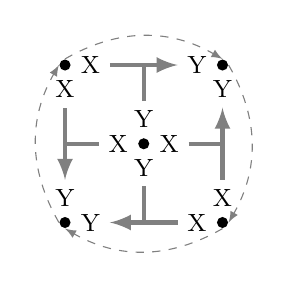
\begin{tikzpicture}
                \node[circle, fill, minimum size =4, inner sep = 0, label={[name=bottomLeftY]right:{\small Y}}, label={[name=bottomLeftY2]above:{\small Y}}](BL) at (-1,-1) {};
                \node[circle, fill, minimum size =4, inner sep = 0, label={[name=topLeftX]below:\small X}, label={[name=topLeftX2]right:\small X}](TL) at (-1,1) {};
                \node[circle, fill, minimum size =4, inner sep = 0, label={[name=bottomrightX]left:\small X},  label={[name=bottomrightX2]above:\small X}](BR) at (1,-1) {};
                \node[circle, fill, minimum size =4, inner sep = 0, label={[name=toprightY]left:\small Y}, label={[name=toprightY2]below:\small Y}](TR) at (1,1) {};
                \node[circle, fill, minimum size =4, inner sep = 0, label={[name=centreX1]left:\small X}, label={[name=centreX2]right:\small X},label={[name=centreY1]below:\small Y}, label={[name=centreY2]above:\small Y}] at (0,0) {};

                                \draw[ultra thick, latex-, gray] (bottomLeftY.east) -- node [midway](BL2BR){} (bottomrightX.west);
                                
                                \draw[ultra thick, -, gray] (centreY1.south) -- (BL2BR.center);
                                \draw[ultra thick, latex-, gray] (bottomLeftY2.north) --  node [midway](BL2TL){} (topLeftX.south);
                                \draw[ultra thick, -latex, gray] (topLeftX2.east) --  node [midway](TL2TR){} (toprightY.west);
                                \draw[ultra thick, -latex, gray] (bottomrightX2.north) --  node [midway](BR2TR){} (toprightY2.south);
                                 \draw[ultra thick, -, gray] (centreY2.north) -- (TL2TR.center);

                                  \draw[ultra thick, -, gray] (centreX1.west) -- (BL2TL.center);

                                   \draw[ultra thick, -, gray] (centreX2.east) -- (BR2TR.center);
                                   \draw[dashed,-latex, gray, label=left:{-1} ] (BL.west)  to[bend left] (TL.west);
                                   \draw[dashed,-latex, gray] (BR.south) to[bend left](BL.south);
                                   \draw[dashed,-latex, gray] (TL.north) to[bend left](TR.north);
                                   \draw[dashed,-latex, gray, label=right:{-1}] (TR.east) to[bend left](BR.east);
                


        \end{tikzpicture}
        \fcaption{\label{faceloops}}
        \end{figure}
\begin{equation}
                E_{ij} = \begin{cases}
                        X_i Y_j X_{f(i,j)} & (i,j) \text{ oriented downwards}\\
                        -X_i Y_j X_{f(i,j)} & (i,j) \text{ oriented upwards}\\
                        X_i Y_j Y_{f(i,j)} & (i,j) \text{ horizontal}\\
                \end{cases}
        \end{equation}
        with the last term ignored if the edge lies on a boundary with no adjacent face qubit. Also map the vertex operators to:
        \begin{equation}
                V_j = Z_j
        \end{equation}
        These satisfy the anti-commutation relations as shown below:
        \begin{equation}
                \{E_{jk}, V_j\} = \begin{cases} \{ X_j Y_k X_{f(j,k)}, Z_j\}\\
-\{ X_j Y_k X_{f(j,k)}, Z_j\}\\
\{X_j Y_k Y_{f(j,k)}, Z_j \}
\end{cases}= \begin{cases} 
\{X_j, Z_j\}  Y_k X_{f(j,k)}\\
-\{X_j, Z_j\}  Y_k X_{f(j,k)}\\
\{X_j, Z_j\}  Y_k Y_{f(j,k)}\\
\end{cases} = 0
        \end{equation}
        \begin{equation}
                \{E_{ij}, E_{jk}\} = \begin{cases}
                        \{ X_i Y_j X_{f(i,j)}, X_j Y_k X_{f(j,k)} \} & (i,j) \text{ and } (j,k) \text{ oriented downwards (1)}\\
                        \{ -X_i Y_j X_{f(i,j)}, X_j Y_k X_{f(j,k)}\} & (i,j) \text{ oriented upwards and } (j,k) \text{ oriented downwards (2) }\\
                        \{ X_i Y_j Y_{f(i,j)} , X_j Y_k X_{f(j,k)}\} & (i,j) \text{ oriented horizontal and } (j,k) \text{ oriented downwards (3)} \\
                        \{ X_i Y_j X_{f(i,j)}, -X_j Y_k X_{f(j,k)} \} & (i,j) \text{ oriented downwards and } (j,k) \text{ oriented upwards (4)}\\
                        \{ -X_i Y_j X_{f(i,j)}, -X_j Y_k X_{f(j,k)}\} & (i,j) \text{ and } (j,k) \text{ oriented upwards (5)} \\
                        \{ X_i Y_j Y_{f(i,j)} , -X_j Y_k X_{f(j,k)} \} & (i,j) \text{ oriented horizontal and } (j,k) \text{ oriented upwards (6)} \\
                        \{ X_i Y_j X_{f(i,j)}, X_j Y_k Y_{f(j,k)} \} & (i,j) \text{ oriented downwards and } (j,k) \text{ oriented horizontal (7)}\\
                        \{ -X_i Y_j X_{f(i,j)}, X_j Y_k Y_{f(j,k)}\} & (i,j) \text{ oriented upwards and } (j,k) \text{ oriented horizontal (8)} \\
                        \{ X_i Y_j Y_{f(i,j)} , X_j Y_k Y_{f(j,k)} \} & (i,j) \text{ and } (j,k) \text{ oriented horizontal (9)} \\
                        \end{cases} 
        \end{equation}
        \begin{equation}
\{E_{ij}, E_{jk}\} = \begin{cases}
        \{Y_j,X_j\} Y_j X_{f(i,j)} Y_k X_{f(j,k)} & (1) \text{ or } (5)\\
        \{  Y_j Y_{f(i,j)} , X_j  X_{f(i,j)}\} X_iY_k & (3) \text{ and } f(i,j) = f(j,k)\\
        \{  Y_j X_{f(i,j)} , X_j  Y_{f(i,j)}\} X_iY_k & (7) \text{ and } f(i,j) = f(j,k)\\
\{ Y_j , X_j  \} X_iY_k Y_{f(i,j)} X_{f(j,k)} & (3) \text{ or } (7) \text{ and } f(i,j) \neq f(j,k)\\
-\{  Y_j Y_{f(i,j)} , X_j  X_{f(i,j)}\} X_iY_k & (6) \text{ and } f(i,j) = f(j,k)\\
-\{  Y_j X_{f(i,j)} , X_j  Y_{f(i,j)}\} X_iY_k & (8) \text{ and } f(i,j) = f(j,k)\\
-\{ Y_j , X_j  \} X_iY_k Y_{f(i,j)} X_{f(j,k)} & (6) \text{ or } (8)  \text{ and } f(i,j) \neq f(j,k)\\
\{X_i Y_j Y_{f(i,j)}, X_j Y_i Y_{f(i,j)} \} & (9) \text{ and } f(i, j) = f(j,k) \\
\{Y_j, X_j\} X_i Y_{f(i,j)} Y_k Y_{f(j,k}} & (9) \text{ and } f(i,j) \neq f(j,k)
\end{cases}
        \end{equation}
Therefore, as $\{Y_j, X_j\} = 0$, we have $\{E_{ij}, E_{jk}\} = 0$ for $f(i,j) \neq f(j,k)$. So any directed edges that meet head to tail anti-commute.
\\\\
        It is necessary to introduce a sign change into the definition of the vertical edge operators depending on orientation so the loops around the black faces equal 1 (and so satisfy the loop condition). \\\\
        Derby-Klassen have developed a design technique for compact fermionic encoding. First you take an undirected graph, then start assigning arrows to it. You then assign qubit operators to every arrow with a X operator at the head of every arrow and a Y operator at the tail. These will automatically anticommute with the Z vertex operator at every mode, and they will anticommute with each other if they are head to tail. However, they will commute with each other if they meet tial to tail or head to head and we want them to anticommute so we add an ancilla qubit to produce this behaviour. For every pair of qubits that commute and we want to anticommute assign a common ancilla and have them act with X and Y respectively. In some instances we can use this qubits for multiple pairs of edges as on the square lattice without breaking the existing commutation and anticommutation rules. Got all this insight from the video. If every $e_{ij}$ anticommutes with $e_{rs}$ then it will anticommute with $e_{sr}$ as $e_{rs} = e_{sr}$, so we only need to consider a directed graph.

        \section{Fermionic Enumeration}\label{fermionic-enumeration_section}
\section{Relative performance}\label{comparision_section}
Talk about how the long strings of Z increase the depth as it makes it hard to decompose in parallel



        \pagebreak
\section{Introduction}        
The journal of {\it Quantum Information and Computation},
for both on-line and in-print editions,
will be produced by using the latex files of manuscripts
provided by the authors. It is therefore essential that the manuscript 
be in its final form, and in the format designed for the journal 
because there will be no futher editing. The authors are strongly encouraged 
to use Rinton latex template to prepare their manuscript. Or, the authors 
should please follow the instructions given here if they prefer to use other 
software. In the latter case, the authors ought to
provide a postscript file of their paper for publication.

\section{Text}
\noindent
Contributions are to be in English. Authors are encouraged to
have their contribution checked for grammar.  
Abbreviations are allowed but should be spelt
out in full when first used. 

\setcounter{footnote}{0}
\renewcommand{\thefootnote}{\alph{footnote}}

The text is to be typeset in 10 pt Times Roman, single spaced
with baselineskip of 13 pt. Text area (excluding running title)
is 5.6 inches across and 8.0 inches deep.
Final pagination and insertion of running titles will be done by
the editorial. Number each page of the manuscript lightly at the
bottom with a blue pencil. Reading copies of the paper can be
numbered using any legible means (typewritten or handwritten).

\section{Headings}
\noindent
Major headings should be typeset in boldface with the first
letter of important words capitalized.

\subsection{Sub-headings}
\noindent
Sub-headings should be typeset in boldface italic and capitalize
the first letter of the first word only. Section number to be in
boldface roman.

\subsubsection{Sub-subheadings}
\noindent
Typeset sub-subheadings in medium face italic and capitalize the
first letter of the first word only. Section number to be in
roman.

\subsection{Numbering and Spacing}
\noindent
Sections, sub-sections and sub-subsections are numbered in
Arabic.  Use double spacing before all section headings, and
single spacing after section headings. Flush left all paragraphs
that follow after section headings.

\subsection{Lists of items}
\noindent
Lists may be laid out with each item marked by a dot:
\begin{itemlist}
 \item item one,
 \item item two.
\end{itemlist}
Items may also be numbered in lowercase roman numerals:
\begin{romanlist}
 \item item one
 \item item two
          \begin{alphlist}
          \item Lists within lists can be numbered with lowercase
              roman letters,
          \item second item.
          \end{alphlist}
\end{romanlist}

\section{Equations}
\noindent
Displayed equations should be numbered consecutively in each
section, with the number set flush right and enclosed in
parentheses.

\begin{equation}
\mu(n, t) = {
\sum^\infty_{i=1} 1(d_i < t, N(d_i) = n) \over \int^t_{\sigma=0} 1(N(\sigma) 
= n)d\sigma}\,. \label{this}
\end{equation}

Equations should be referred to in abbreviated form,
e.g.~``Eq.~(\ref{this})'' or ``(2)''. In multiple-line
equations, the number should be given on the last line.

Displayed equations are to be centered on the page width.
Standard English letters like x are to appear as $x$
(italicized) in the text if they are used as mathematical
symbols. Punctuation marks are used at the end of equations as
if they appeared directly in the text.

\vspace*{12pt}
\noindent
{\bf Theorem~1:} Theorems, lemmas, etc. are to be numbered
consecutively in the paper. Use double spacing before and after
theorems, lemmas, etc.

\vspace*{12pt}
\noindent
{\bf Proof:} Proofs should end with \square\,.

\section{Illustrations and Photographs}
\noindent
Figures are to be inserted in the text nearest their first
reference. The postscript files of figures can be imported by using
the commends used in the examples here.

\begin{figure} [htbp]
%\vspace*{13pt}
\centerline{\epsfig{file=fig1.eps, width=8.2cm}} %100 percent
\vspace*{13pt}
\fcaption{\label{motion}figure caption goes here.}
\end{figure}

Figures are to be sequentially numbered in Arabic numerals. The
caption must be placed below the figure. Typeset in 8 pt Times
Roman with baselineskip of 10~pt. Use double spacing between a
caption and the text that follows immediately.

Previously published material must be accompanied by written
permission from the author and publisher.

\section{Tables}
\noindent
Tables should be inserted in the text as close to the point of
reference as possible. Some space should be left above and below
the table.

Tables should be numbered sequentially in the text in Arabic
numerals. Captions are to be centralized above the tables.
Typeset tables and captions in 8 pt Times Roman with
baselineskip of 10 pt.

\vspace*{4pt}   %only when needed
\begin{table}[hb]
\tcaption{Number of tests for WFF triple NA = 5, or NA = 8.}
\centerline{\footnotesize NP}
\centerline{\footnotesize\smalllineskip
\begin{tabular}{l c c c c c}\\
\hline
{} &{} &3 &4 &8 &10\\
\hline
{} &\phantom03 &1200 &2000 &\phantom02500 &\phantom03000\\
NC &\phantom05 &2000 &2200 &\phantom02700 &\phantom03400\\
{} &\phantom08 &2500 &2700 &16000 &22000\\
{} &10 &3000 &3400 &22000 &28000\\
\hline\\
\end{tabular}}
\end{table}

If tables need to extend over to a second page, the continuation
of the table should be preceded by a caption, e.g.~``({\it Table
2. Continued}).''

\section{References Cross-citation}
\noindent
References cross-cited in the text are to be numbered consecutively in
Arabic numerals, in the order of first appearance. They are to
be typed in brackets such as \cite{first}  and \cite{cal, niel, mar}.
%superscripts after punctuation marks,
%e.g.~``$\ldots$ in the statement.$^5$''.

\section{Sections Cross-citation}\label{sec:abc}
\noindent
Sections and subsctions can be cross-cited in the text by using the latex command
shown here. In Section~\ref{sec:abc}, we discuss ....
%\newpage

\section{Footnotes}
\noindent
Footnotes should be numbered sequentially in superscript
lowercase Roman letters.\fnm{a}\fnt{a}{Footnotes should be
typeset in 8 pt Times Roman at the bottom of the page.}

\nonumsection{Acknowledgements}
\noindent
We would thank ...

\nonumsection{References}
\noindent
References are to be listed in the order cited in the text.
For each cited work, include all the authors' names, year of the work, title,
place where the work appears.
Use the style shown in the following examples. For journal names,
use the standard abbreviations. Typeset references in 9 pt Times
Roman.
\begin{thebibliography}{000}
        \bibitem{feynmann} Feynman, R.P.. {\it Simulating physics with computers}. International Journal of Theoretical Physics 1982;21(6-7):467–488. \url{doi:10.1007/bf02650179}.
        \bibitem{originalJordanWigner} Pascual Jordan and Eugene Wigner. {\it  {\"U}ber das Paulische {\"A}quivalenzverbot}. Zeitschrift fur Physik, 47(9-10):631{651, September 1928.
                \bibitem{fermionicEncoding} Chiew, M. and Strelchuk, S.. {\it Optimal Fermion-Qubit Mappings}. ArXiv:2110.12792 [Quant-Ph], 25 October 2021. \url{http://arxiv.org/abs/2110.12792}
                \bibitem{vqe}
                Tilly, Jules, Hongxiang Chen, Shuxiang Cao, Dario Picozzi, Kanav Setia, Ying Li, Edward Grant, et al. {\it The Variational Quantum Eigensolver: A Review of Methods and Best Practices}. ArXiv:2111.05176 [Quant-Ph], 9 November 2021. \url{http://arxiv.org/abs/2111.05176} \textbf{look for journal version}
                \bibitem{chemistryReview} McArdle, Sam, Suguru Endo, Alán Aspuru-Guzik, Simon C. Benjamin, and Xiao Yuan. {\it Quantum Computational Chemistry}. Reviews of Modern Physics 92, no. 1 (30 March 2020): 015003. \url{https://doi.org/10.1103/RevModPhys.92.015003}.
                \bibitem{nielsenChuang} Nielsen, M.A., Chuang, I.L.. {\it Quantum Computation and Quantum Information}. Cambridge: Cambridge University Press; 2009. ISBN
                \bibitem{seeley} Seeley, Jacob T., Martin J. Richard, and Peter J. Love. {\it The Bravyi-Kitaev Transformation for Quantum Computation of Electronic Structure}. The Journal of Chemical Physics 137, no. 22 (14 December 2012): 224109. \url{https://doi.org/10.1063/1.4768229}.

9780511976667. doi:10.1017/cbo9780511976667.
\bibitem{suzuki} Suzuki, Masuo. {\it Generalized Trotter’s Formula and Systematic Approximants of Exponential Operators and Inner Derivations with Applications to Many-Body Problems}. Communications in Mathematical Physics 51, no. 2 (June 1976): 183–90. \url{https://doi.org/10.1007/BF01609348}.
\bibitem{bravyikitaev} Bravyi, Sergey, and Alexei Kitaev. {\it Fermionic Quantum Computation}. Annals of Physics 298, no. 1 (May 2002): 210–26. \url{https://doi.org/10.1006/aphy.2002.6254}.
\bibitem{tranter2018} Tranter, Andrew, Peter J. Love, Florian Mintert, and Peter V. Coveney. {\it A Comparison of the Bravyi-Kitaev and Jordan-Wigner Transformations for the Quantum Simulation of Quantum Chemistry}. Journal of Chemical Theory and Computation 14, no. 11 (13 November 2018): 5617–30. \url{https://doi.org/10.1021/acs.jctc.8b00450}.
\bibitem{operatorLocality} Havlíček, Vojtěch, Matthias Troyer, and James D. Whitfield. {\it Operator Locality in Quantum Simulation of Fermionic Models}. Physical Review A 95, no. 3 (29 March 2017): 032332. \url{https://doi.org/10.1103/PhysRevA.95.032332}.
\bibitem{superfast} Setia, Kanav, Sergey Bravyi, Antonio Mezzacapo, and James D. Whitfield. {\it Superfast Encodings for Fermionic Quantum Simulation}. Physical Review Research 1, no. 3 (18 October 2019): 033033. \url{https://doi.org/10.1103/PhysRevResearch.1.033033}.
\bibitem{derbyklassen} Derby, Charles, and Joel Klassen. {\it A Compact Fermion to Qubit Mapping}. Physical Review B 104, no. 3 (8 July 2021): 035118. \url{https://doi.org/10.1103/PhysRevB.104.035118}.
\bibitem{derbyklassen2} Derby, Charles, and Joel Klassen. {\it A Compact Fermion to Qubit Mapping Part 2: Alternative Lattice Geometries}. ArXiv:2101.10735 [Quant-Ph], 26 January 2021. http://arxiv.org/abs/2101.10735.
                \bibitem{first}
P. Horodecki and R. Horodecki (2001), {\it Distillation and bound entanglement},
Quantum Inf. Comput., Vol.1, pp. 045-075.

\bibitem{cal}
R. Calderbank and P. Shor (1996), {\it Good quantum error
       correcting codes exist},
Phys. Rev. A, 54, pp. 1098-1106.

\bibitem{niel}
M.A. Nielsen and J. Kempe (2001), {\it Separable states are
more disordered globally than locally}, quant-ph/0105090.

\bibitem{mar}
A.W. Marshall and I. Olkin (1979), {\it Inequalities: theory of majorization and its applications},
Academic Press (New York).
\end{thebibliography}

\appendix

\noindent
Appendices should be used only when absolutely necessary. They
should come after the References. If there is more than one
appendix, number them alphabetically. Number displayed equations
occurring in the Appendix in this way, e.g.~(\ref{that}), (A.2),
etc.
\begin{equation}
\langle\hat{O}\rangle=\int\psi^*(x)O(x)\psi(x)d^3x~. 
\label{that}
\end{equation}
\end{document}

